%%%%%%%%%%%%%%%%%%%%%%%%%%%%%%%%%%%%%%%%%
% Beamer Presentation
% LaTeX Template
% Version 1.0 (10/11/12)
%
% This template has been downloaded from:
% http://www.LaTeXTemplates.com
%
% License:
% CC BY-NC-SA 3.0 (http://creativecommons.org/licenses/by-nc-sa/3.0/)
%
%%%%%%%%%%%%%%%%%%%%%%%%%%%%%%%%%%%%%%%%%

%----------------------------------------------------------------------------------------
%	PACKAGES AND THEMES
%----------------------------------------------------------------------------------------

\documentclass[UTF8]{ctexbeamer}

\usepackage{hyperref}
\hypersetup{
  colorlinks=true,
  linkcolor=red,
  anchorcolor=blue,
  citecolor=green
}

\mode<presentation> {

% The Beamer class comes with a number of default slide themes
% which change the colors and layouts of slides. Below this is a list
% of all the themes, uncomment each in turn to see what they look like.

%\usetheme{default}
%\usetheme{AnnArbor}
%\usetheme{Antibes}
%\usetheme{Bergen}
%\usetheme{Berkeley}
%\usetheme{Berlin}
%\usetheme{Boadilla}
%\usetheme{CambridgeUS}
%\usetheme{Copenhagen}
%\usetheme{Darmstadt}
%\usetheme{Dresden}
%\usetheme{Frankfurt}
%\usetheme{Goettingen}
%\usetheme{Hannover}
%\usetheme{Ilmenau}
%\usetheme{JuanLesPins}
%\usetheme{Luebeck}
\usetheme{Madrid}
%\usetheme{Malmoe}
%\usetheme{Marburg}
%\usetheme{Montpellier}
%\usetheme{PaloAlto}
%\usetheme{Pittsburgh}
%\usetheme{Rochester}
%\usetheme{Singapore}
%\usetheme{Szeged}
%\usetheme{Warsaw}

% As well as themes, the Beamer class has a number of color themes
% for any slide theme. Uncomment each of these in turn to see how it
% changes the colors of your current slide theme.

%\usecolortheme{albatross}
%\usecolortheme{beaver}
%\usecolortheme{beetle}
%\usecolortheme{crane}
%\usecolortheme{dolphin}
%\usecolortheme{dove}
%\usecolortheme{fly}
%\usecolortheme{lily}
%\usecolortheme{orchid}
%\usecolortheme{rose}
%\usecolortheme{seagull}
%\usecolortheme{seahorse}
%\usecolortheme{whale}
%\usecolortheme{wolverine}

%\setbeamertemplate{footline} % To remove the footer line in all slides uncomment this line
%\setbeamertemplate{footline}[page number] % To replace the footer line in all slides with a simple slide count uncomment this line

%\setbeamertemplate{navigation symbols}{} % To remove the navigation symbols from the bottom of all slides uncomment this line
}

\usepackage{graphicx} % Allows including images
\graphicspath{{./figs/}}
\usepackage{booktabs} % Allows the use of \toprule, \midrule and \bottomrule in tables
\usepackage{longtable}

% Fonts
% \usepackage{libertine}
% \setmonofont{Courier}
\setCJKsansfont[ItalicFont=Noto Serif CJK SC Black, BoldFont=Noto Sans CJK SC Black]{Noto Sans CJK SC}

%----------------------------------------------------------------------------------------
%	TITLE PAGE
%----------------------------------------------------------------------------------------

\title[第1讲]{第1讲 :操作系统概述} % The short title appears at the bottom of every slide, the full title is only on the title page
\subtitle{第八节:OS实验概述}
\author{向勇、陈渝} % Your name
\institute[清华大学] % Your institution as it will appear on the bottom of every slide, may be shorthand to save space
{
清华大学计算机系 \\ % Your institution for the title page
\medskip
\textit{xyong,yuchen@tsinghua.edu.cn} % Your email address
}
\date{\today} % Date, can be changed to a custom date

\begin{document}

\begin{frame}
\titlepage % Print the title page as the first slide
\end{frame}

%\begin{frame}
%\frametitle{提纲} % Table of contents slide, comment this block out to remove it
%\tableofcontents % Throughout your presentation, if you choose to use \section{} and \subsection{} commands, these will automatically be printed on this slide as an overview of your presentation
%\end{frame}
%
%%----------------------------------------------------------------------------------------
%%	PRESENTATION SLIDES
%%----------------------------------------------------------------------------------------
%
%%------------------------------------------------
%\section{第八节:OS实验概述} % Sections can be created in order to organize your presentation into discrete blocks, all sections and subsections are automatically printed in the table of contents as an overview of the talk
%%------------------------------------------------


\begin{frame}

\frametitle{OS实验概述}

\begin{itemize}
\item 设计思路
    \begin{itemize}
    \item 采用小巧全面的操作系统ucore并进行改进,需要覆盖操作系统的关键点,为此增加:
    \begin{itemize}
        \item 外设:I/O管理/中断管理
        \item 内存:虚存管理/页表/缺页处理/页替换算法
        \item CPU:进程管理/调度器算法
        \item 并发:信号量实现和同步互斥应用
        \item 存储:文件系统+磁盘驱动
    \end{itemize}
    \item 完整代码量控制在10000行以内
    \item 提供实验讲义和源码分析文档
    \end{itemize}
\end{itemize}

\end{frame}


\begin{frame}
	
	\frametitle{OS实验内容}

	\begin{columns}
    \begin{column}{.35\linewidth}
    OS实验内容
	\begin{enumerate}
	    \item OS启动/中断/异常
		\item 物理内存管理
		\item 虚拟内存管理	
		\item 内核模式线程管理
		\item 用户模式进程管理
		\item 处理器调度
		\item 多处理与同步互斥
		\item 文件系统
	\end{enumerate}
	\end{column}
	
	\begin{column}{.7\linewidth}
	\begin{figure}
		\centering
		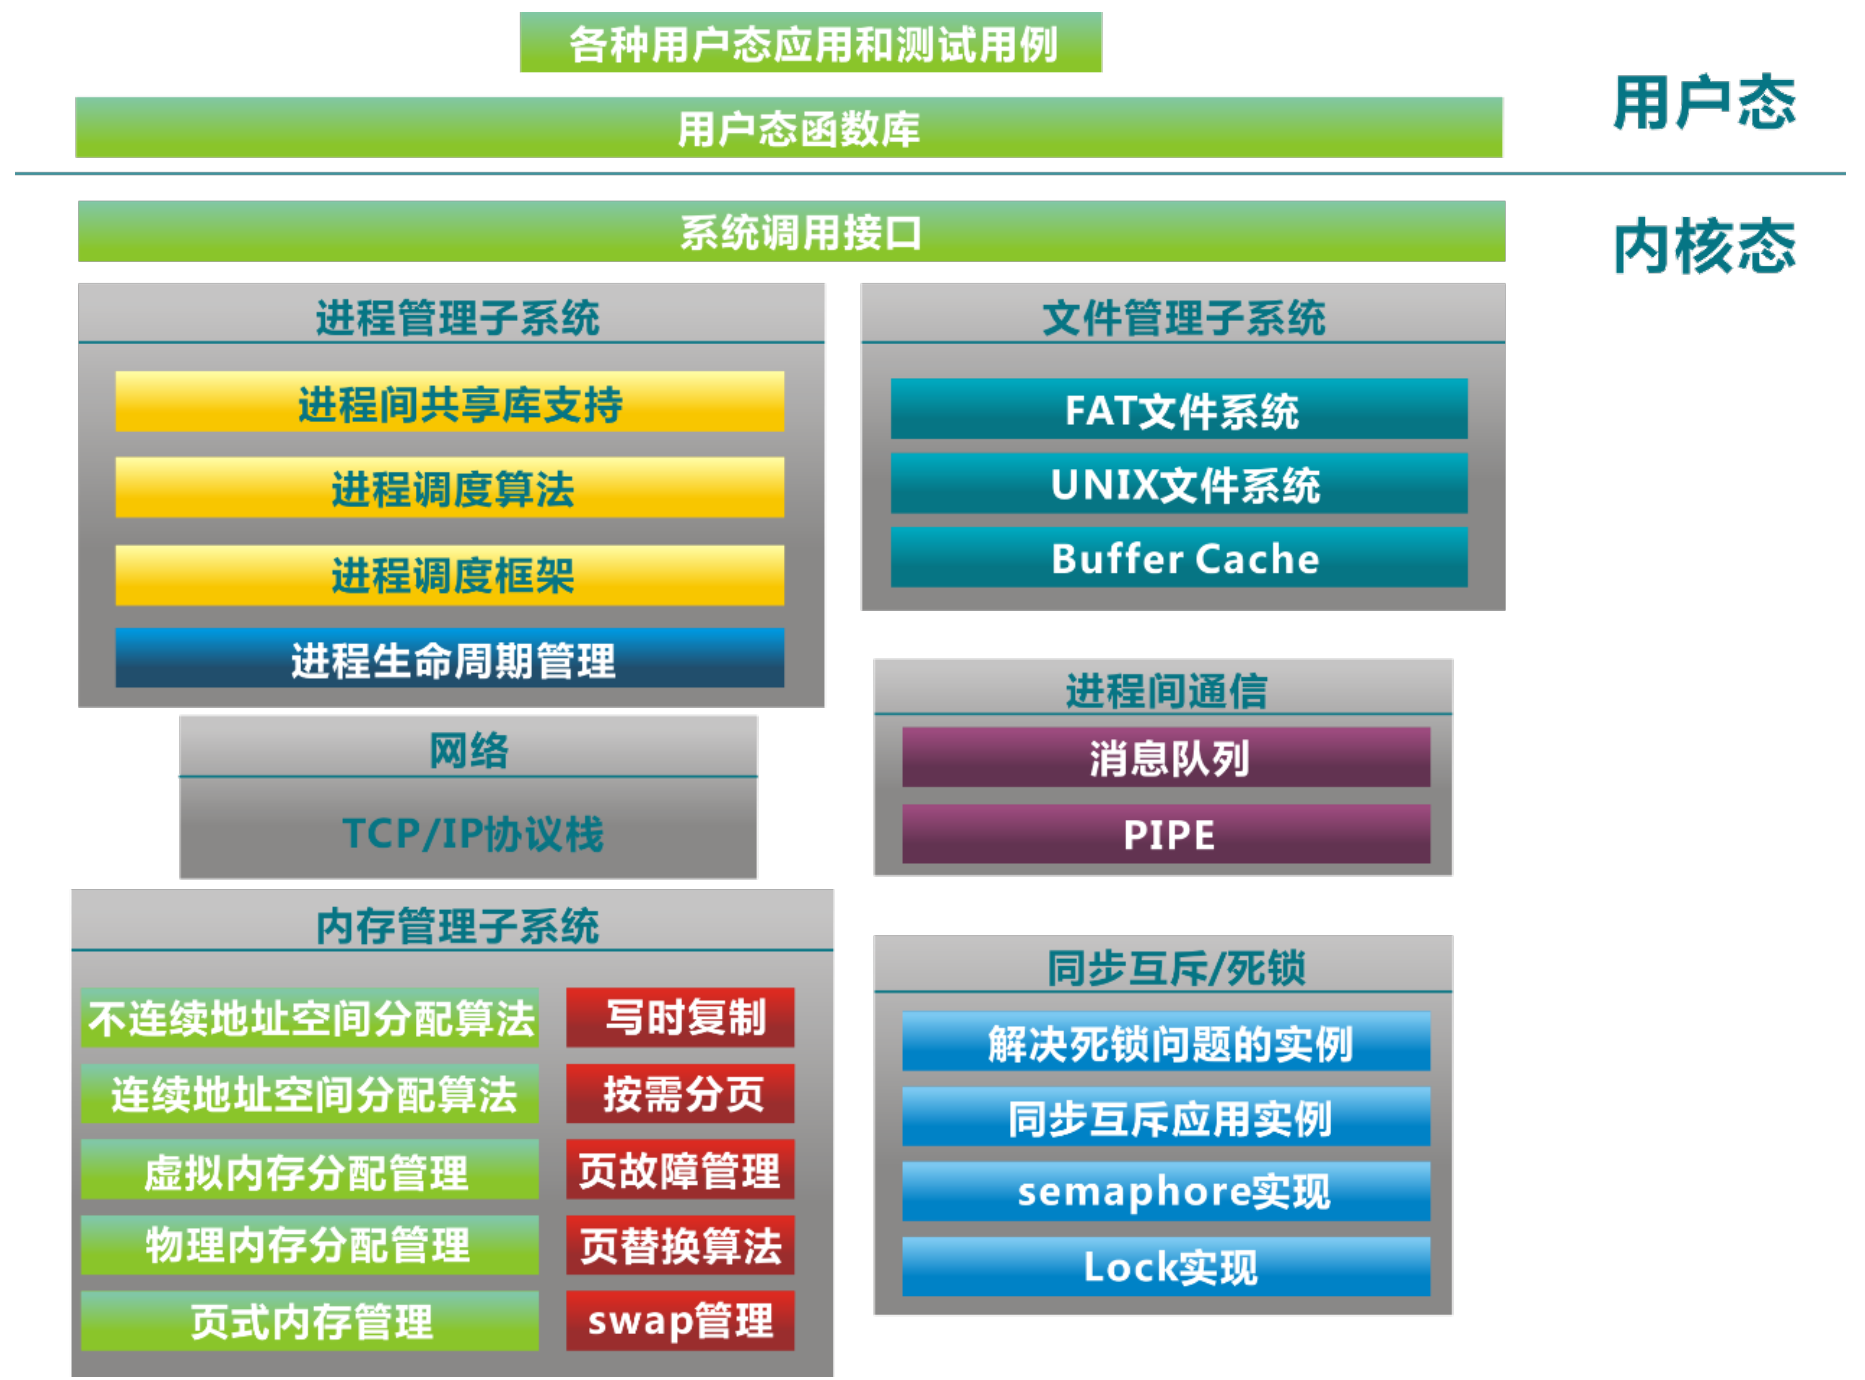
\includegraphics[width=1.0\linewidth]{oslab-overview}
		\caption{OS实验框架}
	\end{figure}
	\end{column}
	\end{columns}
\end{frame}


\begin{frame}
\frametitle{OS实验内容}
\framesubtitle{lab1}
\begin{block}{Lab1:  Bootloader/Interrupt/Debug}
启动操作系统的bootloader,了解操作系统启动前的
状态和要做的事,了解运行操作系统的硬件支持,
操作系统如何加载到内存中,理解两类中断--“外设中断”,   
“异常”等。
\end{block}

\begin{itemize}
    \item 编译运行直接与硬件交互的系统程序
    \item 启动bootloader的过程
    \item 实现中断处理机制
    \item 输出字符的方法
    \item 调试系统程序的方法
\end{itemize}
    
\end{frame}


\begin{frame}
\frametitle{OS实验内容}
\framesubtitle{lab2}

\begin{block}{Lab2:  物理内存管理}
理解分页模式,了解操作系统如何管理连续空间的物理内存。
\end{block}

\begin{itemize}
    \item 理解内存地址的转换和保护
    \item 实现页表的建立和使用方法
    \item 实现物理内存的管理方法
    \item 了解常用的减少碎片的方法
\end{itemize}

\end{frame}

\begin{frame}
\frametitle{OS实验内容}
\framesubtitle{lab3}

\begin{block}{Lab3:虚拟内存管理}
了解页表机制和换出(swap)机制,以及中断-“故障中断”、
缺页故障处理等,基于页的内存替换算法。
\end{block}

\begin{itemize}
    \item 理解换页的软硬件协同机制
    \item 实现虚拟内存的Page Fault异常处理
    \item 实现页替换算法
\end{itemize}

\end{frame}

\begin{frame}
\frametitle{OS实验内容}
\framesubtitle{lab4}

\begin{block}{Lab4: 内核模式线程管理}
了解如果利用CPU来高效地完成各种工作的设计与实现基础,
如何创建相对与用户进程更加简单的内核态线程,
如何对内核线程进行动态管理等。
\end{block}

\begin{itemize}
    \item 建立内核线程的关键信息
    \item 实现内核线程的管理方法
\end{itemize}

\end{frame}


\begin{frame}
\frametitle{OS实验内容}
\framesubtitle{lab5}

\begin{block}{Lab5: 用户模式进程管理}
了解用户态进程创建、执行、切换和结束的动态管理过程,
了解在用户态通过系统调用得到内核态的内核服务的过程。
\end{block}

\begin{itemize}
    \item 建立用户进程的关键信息
    \item 实现用户进程管理
    \item 分析进程和内存管理的关系
    \item 实现系统调用的处理过程
\end{itemize}

\end{frame}

\begin{frame}
\frametitle{OS实验内容}
\framesubtitle{lab6}

\begin{block}{Lab6:调度}
理解操作系统的调度过程和调度算法。
\end{block}

\begin{itemize}
    \item 熟悉系统调度器框架,以及内置的 Round-Robin 调度算法
    \item 基于调度器框架实现一个调度器算法
\end{itemize}

\end{frame}


\begin{frame}
\frametitle{OS实验内容}
\framesubtitle{lab7}

\begin{block}{Lab7:同步互斥}
了解进程间如何进行信息交换和共享,并了解同步互斥的具体实现
以及对系统性能的影响,研究死锁产生的原因,以及如何避免死锁。
\end{block}

\begin{itemize}
    \item 熟悉 同步互斥的实现机制
    \item 理解基本的spinlock、semphpore、condition variable的实现
    \item 实现基于各种同步机制的同步问题。
\end{itemize}

\end{frame}


\begin{frame}
\frametitle{OS实验内容}
\framesubtitle{lab8}

\begin{block}{Lab8:文件系统}
了解文件系统的具体实现,与进程管理等的关系,
了解缓存对操作系统IO访问的性能改进,了解虚拟文件系统(VFS)、
buffer cache和disk driver之间的关系。
\end{block}

\begin{itemize}
    \item 掌握基本的文件系统系统调用的实现方法
    \item 了解一个基于inode方式的SFS文件系统的设计与实现
    \item 了解文件系统抽象层-VFS的设计与实现
\end{itemize}

\end{frame}


\begin{frame}
\frametitle{OS实验内容}
\framesubtitle{labX}

\begin{block}{LabX:大实验}
前提:已经完成基本实验 \\
尝试完成一些有一定挑战性且有趣的OS实验。
\end{block}

\begin{itemize}
    \item 重新设计zircon操作系统
    \item 在一个OS(如Linux)实现一个Hypervisor
    \item OS直接支持运行被隔离的应用程序
    \item 支持动态更新的OS
    \item 驱动程序运行在用户态的OS
    \item 支持标签化CPU的OS
    \item 一个可验证正确性的OS
    \item 运行在抽象计算机上可动态调试的OS
\end{itemize}

\end{frame}


\begin{frame}
	\frametitle{OS实验内容}
	\framesubtitle{labX}
	
\begin{longtable}[]{@{}|l|l|@{}}
	\toprule
	选题方向 & 大实验题目\tabularnewline
	\midrule
	\endhead
	RISC-V &
	\href{http://os.cs.tsinghua.edu.cn/oscourse/OS2019spring/projects/g01}{ucore
		on RISC-V}\tabularnewline  \hline
	RISC-V &
	\href{http://os.cs.tsinghua.edu.cn/oscourse/OS2019spring/projects/g02}{简易版
		rcore 开发与教学文档编写 \&\& rcore plus 开发}\tabularnewline \hline
	RISC-V &
	\href{http://os.cs.tsinghua.edu.cn/oscourse/OS2019spring/projects/g05}{FPGA
		上运行 RISC-V rCore 构建路由器}\tabularnewline \hline
	x86\_64 &
	\href{http://os.cs.tsinghua.edu.cn/oscourse/OS2019spring/projects/g04}{对标
		Biscuit OS 真实应用真实网卡及性能测试}\tabularnewline \hline
	x86\_64 &
	\href{http://os.cs.tsinghua.edu.cn/oscourse/OS2019spring/projects/g06}{rCore
		内核可加载模块和动态链接库}\tabularnewline \hline
	MIPS &
	\href{http://os.cs.tsinghua.edu.cn/oscourse/OS2019spring/projects/g03}{第三届全国大学生系统能力培养大赛}\tabularnewline \hline
	Arm &
	\href{http://os.cs.tsinghua.edu.cn/oscourse/OS2019spring/projects/g11}{Python
		(and more) on rCore on RPi}\tabularnewline \hline
	GUI &
	\href{http://os.cs.tsinghua.edu.cn/oscourse/OsTrain2019/g2}{GUI}\tabularnewline \hline
	GUI & \href{http://os.cs.tsinghua.edu.cn/oscourse/OsTrain2019/g3}{适配
		mini GUI}\tabularnewline \hline

	
	\bottomrule
\end{longtable}


\end{frame}



\begin{frame}
	\frametitle{OS实验内容}
	\framesubtitle{labX}
	
	\begin{longtable}[]{@{}|l|l|@{}}
		\toprule
		选题方向 & 大实验题目\tabularnewline
		\midrule
		\endhead
		驱动 &
		\href{http://os.cs.tsinghua.edu.cn/oscourse/OsTrain2019/g4}{IO复用}\tabularnewline \hline
		rust &
		\href{http://os.cs.tsinghua.edu.cn/oscourse/OS2019spring/projects/g08}{Audio
			support for rCore}\tabularnewline \hline
		内核语言 &
		\href{http://os.cs.tsinghua.edu.cn/oscourse/OsTrain2019/g6}{编译原理/操作系统综合实验}\tabularnewline \hline
		错误分析 &
		\href{http://os.cs.tsinghua.edu.cn/oscourse/OS2019spring/projects/g07}{在ucore获得稳定触发竞争条件的漏洞样本}\tabularnewline \hline
		行为分析 &
		\href{http://os.cs.tsinghua.edu.cn/oscourse/OS2019spring/projects/g09}{Program
			Analysis via Memory Access Patterns}\tabularnewline \hline
		微内核 &
		\href{http://os.cs.tsinghua.edu.cn/oscourse/OsTrain2019/g1}{调研Fuchsia的微内核,尝试rcore微内核的修改}\tabularnewline \hline
		内核可加载模块 &
		\href{http://os.cs.tsinghua.edu.cn/oscourse/OsTrain2019/g5}{rethink用户/内核态}\tabularnewline \hline
		模拟器 &
		\href{http://os.cs.tsinghua.edu.cn/oscourse/OS2019spring/projects/g10}{操作系统中常用算法的性能分析及优化}\tabularnewline \hline
		教学实验设计 &
		\href{http://os.cs.tsinghua.edu.cn/oscourse/OsTrain2019/g7}{对简易版rcore的进一步维护和更新}\tabularnewline \hline
		\bottomrule
	\end{longtable}
	

\end{frame}
%----------------------------------------------------------------------------------------

\end{document}
